\documentclass[a4paper, 12pt, titlepage, openany]{book}
\usepackage{BackGround}
\usepackage{varwidth}
\makeindex


\begin{document}
\begin{titlepage}
\begin{center}

\includegraphics[scale=1]{IMGS/copertina}
\\ \huge \textbf{CineMaX\\ \hspace{2mm} manuale utente }
\vspace{3mm}
\\ \normalsize 721086 Francesco Ferrari \\
768081 Nithay Patricia Gomez Silva\\
766922 Pasquale Di Tuccio\\
Luca \\
\vspace{3mm}
Università Degli Studi Dell'Insubria \\
Corso Di Laurea In Informatica, sede di Varese

\end{center}
\end{titlepage}

%\maketitle

\chapter*{Introduzione}
CineMaX è un'applicazione pensata per gestire un cinema monosala della capienza di 200 posti.
In questo documento sono descritte le varie operazioni che possono essere eseguite come ad esempio registrare un nuovo utente, effettuare il login, prenotare posti  in sala per la proiezione di un film e molto altro.

\tableofcontents

\chapter{Requisiti e installazione}
%finchè non c'è l'eseguibile non si può scrivere

\chapter{Tipi di utente}
L'applicazione permette l'utilizzo da parte di di quattro tipi di utente diversi, a seconda del tipo di utente che effettua l'accesso cambiano le operazioni che possono essere eseguite.
Lo username dei clienti è deciso in fase di registrazione, mentre quello dei dipendenti è assegnato dal gestore del cinema secondo  un formato predefinito. \'E possibile registrare i clienti dal terminale, mentre i dipendenti (proiezionisti e biglietttai) devono essere aggiunti a mano dal gestore del cinema.
\section{Utente di tipo guest}
Questo tipo di utente non necessita di registrazione e può solo effettuare la ricerca di una proiezione presente a palinsesto.
\section{Utente di tipo cliente}
Questo tipo di utente rappresenta i clienti del cinema e può
\begin{center}
\begin{varwidth}{\textwidth}
\begin{itemize}
\item[•] effettuare la ricerca di una proiezione e prenotare posti
\item[•] visualizzare le prenotazioni effettuate
\end{itemize}
\end{varwidth}
\end{center} 
\section{Utente di tipo proiezionista}
Questo tipo di utente rappresenta i Proiezionisti del cinema, questo tipo di account può
\begin{center}
\begin{varwidth}{\textwidth}
\begin{itemize}
\item[•] aggiungere una proiezione al palinsesto
\item[•] eliminare una proiezione dal palinsesto
\end{itemize}
\end{varwidth}
\end{center} 
lo username di questo tipo di account è nel formato **PRO[numero] (esempio **PRO1).

\section{Utente di tipo bigliettaio}
Questo tipo di utente rappresenta i Proiezionisti del cinema, questo tipo di account può
\begin{center}
\begin{varwidth}{\textwidth}
\begin{itemize}
\item[•] visualizzare tutte le prenotazioni per la data odierna
\item[•] cercare una prenotazione effettuata da un utente di tipo cliente
\end{itemize}
\end{varwidth}
\end{center} 
lo username di questo tipo di account è nel formato \$\$BIG[numero] (esempio \$\$BIG1).

\chapter{Menù principale}
\begin{figure}[!htbp]
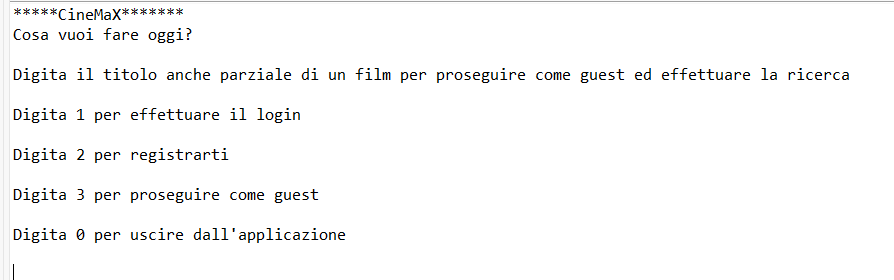
\includegraphics[scale=0.7]{IMGS/menuavvio}
\caption{Il menu principale di CineMaX}
\end{figure}

Ad ogni avvio dell'applicazione viene mostrato il menù principale, che consente all'utente di selezionare l'operazione che desidera eseguire tramite la pressione di un tasto:
%elenchi centrati nella pagina
\begin{center}
\begin{varwidth}{\textwidth}
\begin{itemize}
\item[•] premi il tasto numerico 1 per effettuare il login
\item[•] premi il tasto numerico 2 per effettuare il login
\item[•] premi il tasto numerico 3 per accedere come guest
\end{itemize}
\end{varwidth}
\end{center}

in alternativa è possibile digitare qualsiasi cosa, che verrà interpretata come titolo di un film e il programma inizierà la ricerca di proiezioni con quel titolo anche se parziale; per esempio se si scrive Mons invece che Monsters, inc l'applicazione mostrerà tutte le proiezioni dei film che contengono la parola "Mons" al loro interno, non bisogna preoccuparsi di maiuscole o minuscole nei titoli per CineMaX non fa differenza.

\begin{figure}[!htbp]
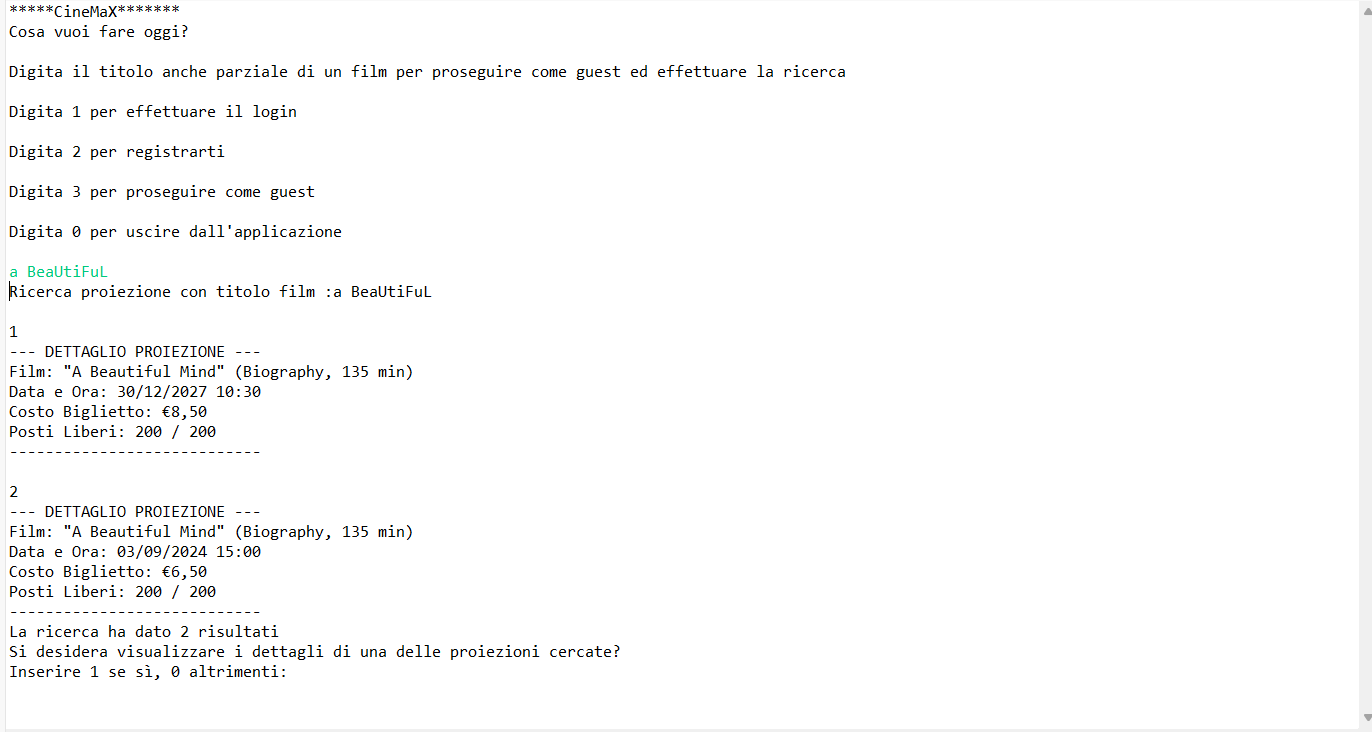
\includegraphics[scale=0.7]{IMGS/ricercadamenuprincipale}
\caption{Esempio di ricerca di un film da menù di avvio, il titolo è stato inserito volutamente incompleto e con maiuscole e minuscole}
\end{figure}

\chapter{Registrazione}
L'applicazione consente la registrazione da terminale di un nuovo account esclusivamente di tipo cliente, per cominciare il processo è necessario premere il tasto 2 nel menù principale.
L'applicazione chiederà di inserire le seguenti informazioni in quest'ordine:
\begin{center}
\begin{varwidth}{\textwidth}
\begin{itemize}
\item[•] nome
\item[•] cognome 
\item[•] data di nascita 
\item[•] città di residenza 
\item[•] username
\item[•] password 
\end{itemize}
\end{varwidth}
\end{center}
nome e cognome devono essere composti da almeno due lettere e non devono contenere numeri o caratteri speciali $(?,!_ ,...)$, la data di nascita dev'essere in formato AAAA-MM-GG, tuttavia il programma riconosce formati di data diversi e li adatta automaticamente; la città di residenza deve contenere almeno una lettera e non contenere numeri o caratteri speciali e lo username deve essere formato da almeno due lettere, mentre la password deve contenere almeno un carattere.
L'applicazione esegue un controllo dell'età e non permette la registrazione di persone con età maggiore o uguale a 125 anni, inoltre se un minorenne sta provando a registrarsi il programma richiede il login con un account di un maggiorenne per poter proseguire il processo.
Se l'utente sbaglia a inserire un campo o se lo username scelto è già in uso compare un messaggio di errore e si viene invitati a riprovare l'inserimento fino a quando non si inserisce un valore valido; se la registrazione va a buon fine viene mostrato un messaggio che contiene l'ID univoco assegnato al nuovo utente.
\begin{figure}[!htbp]
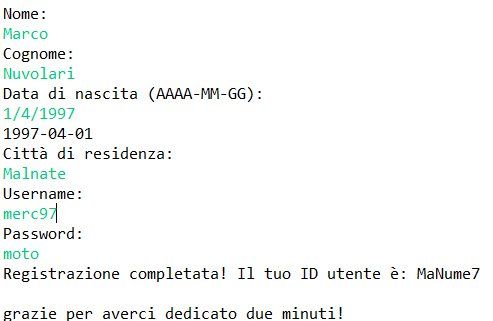
\includegraphics[scale=0.6]{IMGS/registrazioneok}
\caption{Esempio di registrazione andato a buon fine}
\end{figure}

\chapter{Login}
Premendo il tasto 1 nel menù principale si effettua il login all'applicazione, necessario per accedere alle funzionalità collegate al proprio tipo di account.
Per effettuare il login di un account il programma richiede username e password, se il login va a buon fine viene mostrato un messaggio di benvenuto e si accede al menù utente, altrimenti uno di errore e si viene rimandati al menù principale

\begin{figure}[!htbp]
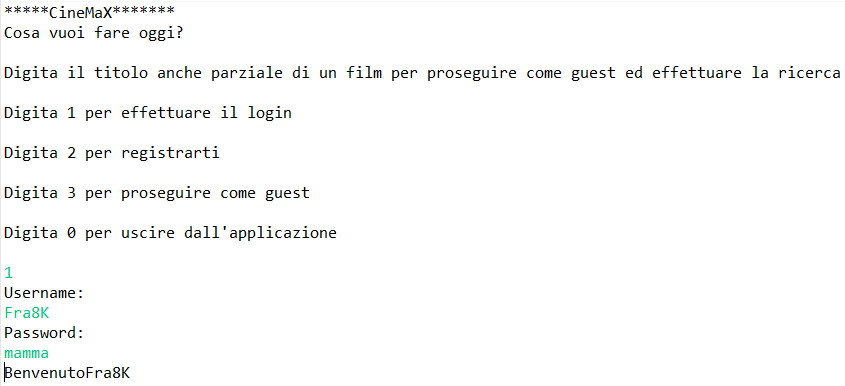
\includegraphics[scale=0.5]{IMGS/loginriuscito}
\caption{Esempio di login andato a buon fine}
\end{figure}

\begin{figure}[!htbp]
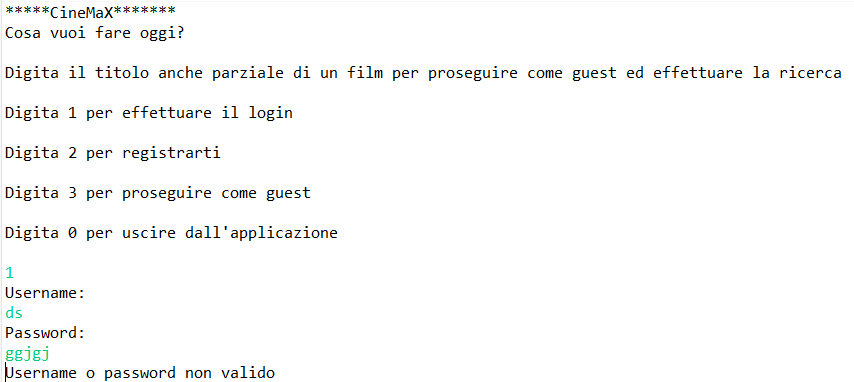
\includegraphics[scale=0.5]{IMGS/loginfallito}
\caption{Esempio di login non andato a buon fine}
\end{figure}

\section{Guest}
Se si decide di proseguire come guest comapre il menù mostrato in figura, in cui è possibile selezionare l'azione da compiere premendo un tasto numerico, qualsiasi altro tasto premuto sarà interpretato come titolo anche parziale di un film e sarà effettuata la ricerca delle proiezioni aventi quel titolo come nel menù principale.
\begin{figure}[!htbp]
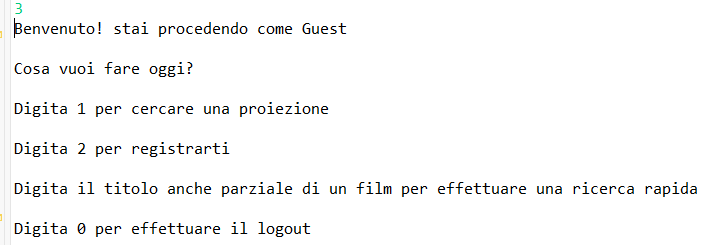
\includegraphics[scale=0.5]{IMGS/menuguest}
\caption{Menù utente guest}
\end{figure}

\section{Cliente}
Se si decide di proseguire come cliente comapre il menù mostrato in figura, in cui è possibile selezionare l'azione da compiere premendo un tasto numerico, qualsiasi altro tasto premuto genera un messaggio di selezione invalida.
\begin{figure}[!htbp]
\centering
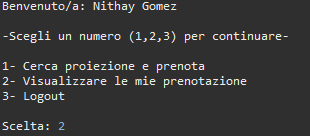
\includegraphics[scale=1]{IMGS/menuutente}
\caption{Menù cliente}
\end{figure}

\section{Proiezionista}
\begin{figure}[!htbp]
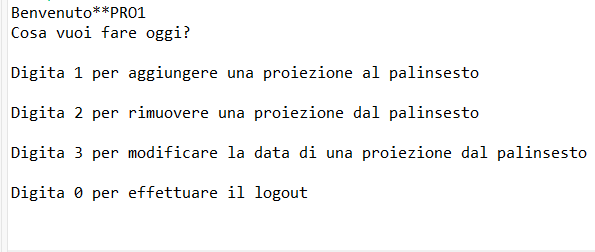
\includegraphics[scale=0.5]{IMGS/menuproiezionista}
\caption{Menù proiezionista}
\end{figure}

\section{Bigliettaio}
\begin{figure}[!htbp]

\includegraphics[scale=0.5]{IMGS/menubigliettaio}
\caption{Menù bigliettaio}
\end{figure}






\end{document}

